\documentclass{article}
\usepackage{iclr2026_conference,times}
\usepackage{amsmath,amssymb}
\usepackage{booktabs}
\usepackage{graphicx}
\usepackage{xcolor}
\definecolor{linkblue}{HTML}{0D4F78}
\usepackage[colorlinks=true, linkcolor=linkblue, citecolor=linkblue, urlcolor=linkblue]{hyperref}
\usepackage{url}
\usepackage{microtype}
\usepackage{enumitem}
\usepackage[most]{tcolorbox}
\setlength{\textfloatsep}{9pt plus 2pt minus 2pt}
\setlength{\floatsep}{8pt plus 2pt minus 2pt}
\setlength{\intextsep}{8pt plus 2pt minus 2pt}

\newtcolorbox{scenariobox}[1]{
  breakable,
  enhanced,
  colback=gray!5,
  colframe=gray!40,
  borderline west={2.2pt}{0pt}{linkblue!70!black},
  coltitle=black,
  colbacktitle=gray!12,
  fonttitle=\sffamily\bfseries\footnotesize,
  fontupper=\footnotesize,
  title={#1},
  boxrule=0.4pt,
  arc=2pt,
  left=7pt, right=7pt, top=5pt, bottom=5pt,
  toptitle=3pt, bottomtitle=3pt
}

\newtcolorbox{promptbox}[1]{
  breakable,
  enhanced,
  colback=linkblue!4,
  colframe=linkblue!35,
  borderline west={2.5pt}{0pt}{linkblue},
  coltitle=linkblue!90!black,
  colbacktitle=linkblue!10,
  fonttitle=\sffamily\bfseries\footnotesize,
  fontupper=\sffamily\footnotesize,
  title={#1},
  boxrule=0.4pt,
  arc=2pt,
  left=7pt, right=7pt, top=5pt, bottom=5pt,
  toptitle=3pt, bottomtitle=3pt
}

\iclrfinalcopy

\title{Sci-TwistBench: Scientific Monoculture in \\ Language Models Asked to \\ Reframe Anomalies}

\author{Joshua Swanson \\
Max Planck Institute for Intelligent Systems \\
\texttt{joshua.swanson@tuebingen.mpg.de}
}

\begin{document}
\maketitle
\lhead{Sci-TwistBench Research Report}

\section{Central Claim}
\label{sec:claim}

Scientific breakthroughs often require transformational creativity, the capacity to revise the problem formulation itself \citep{vanderschaar2026creativity}. We introduce Sci-TwistBench, adapting TwistBench from creative writing to scientific hypothesis generation, to measure one precondition for this capacity in language models. Each task presents a synthetic experimental anomaly with fixed controls that rule out trivial explanations, and asks a model to propose an explanatory hypothesis across repeated runs. We score those hypotheses with LLM judges and group them by causal mechanism. We ask each model explicitly to revise an assumption of the prevailing theory because most models are instruction-tuned and trained to work within the task they are given. We argue that a requested revision is the closest observable proxy for transformational creativity. \citet{vanderschaar2026creativity} call the ability to sustain multiple alternative formulations over time formulation maintenance. This ability requires more than one formulation. We claim that current models produce a reframing when asked but rarely produce more than one. We refer to this as scientific monoculture, following \citet{traberg2026monoculture}. Three findings support the claim. First, seven open-weight and proprietary models produce a valid reframing on at least 91\% of single runs, yet 61\% to 91\% of each model's revisions propose the same causal mechanism. Different models favor largely the same mechanisms. Second, across matched \texttt{OLMo-3} checkpoints, monoculture among valid hypotheses increases most after reasoning distillation, stays flat across later preference and reinforcement stages in reasoning models, and does not increase with scale. Third, of four inference-time methods, only Verbalized Sampling and In-Context Regeneration, which both ask a model for several distinct hypotheses, lower monoculture substantially.

\section{Sci-TwistBench}
\label{sec:benchmark}

\subsection{Adapting TwistBench to Scientific Hypothesis Generation}

Sci-TwistBench adapts TwistBench \citep{schapiro2026twistbench} from literary plot twists to scientific hypothesis generation. TwistBench operationalizes transformational creativity \citep{boden2004creative} by testing whether models write surprising, coherent, realistic, and diverse plot twists that force a reader to reinterpret earlier events. We port this four-axis framework to scientific discovery \citep{vanderschaar2026creativity}. Each anomaly specifies fixed empirical findings, a prevailing theory that fails to explain them, and the implicit assumptions sustaining that theory. Validity on a single run tests whether a model can drop or invert an implicit assumption while respecting every finding and established domain laws. Our prompt requests this revision explicitly, so validity on a single run shows only that a model can revise an assumption when asked. \citet{vanderschaar2026creativity} require that a system initiate the revision itself, which they call endogenous initiation. However, every widely deployed LLM is instruction-tuned and trained to work within the task it is given. We argue that a benchmark cannot observe endogenous initiation directly. The closest available proxy is therefore to request a revision. Each hypothesis revises a modeling assumption, so we treat distinct causal mechanisms as alternative revisions of the problem formulation. Diversity across independent runs is then a precondition for formulation maintenance. A model that returns one default explanation on every run produces only one formulation.

\subsection{Scenarios and Memorization Controls}

We authored 12 synthetic scientific anomaly cases covering four fields (three each in Clinical and Biomedical Science, Physics and Materials, Ecology and Earth Systems, and Economics and Behavioral Science, detailed in Appendix~\ref{app:scenarios}). Each case summarizes a study, states the prevailing theory, reports an unexpected quantitative result, and gives four explicit experimental constraints ($E_1$--$E_4$). For example, one clinical case describes a trial in which an oral drug lowers LDL cholesterol at some hospitals yet fails at the rest despite identical tablet purity, plasma exposure, and patient genetics. These constraints rule out measurement error and simple confounding while leaving room for multiple realistic mechanisms. We also construct four memorization controls to test whether mode collapse merely reflects memorized textbook solutions. Each control pairs a historical case with a transferred case. The historical case is a classic discovery. The transferred case is a structurally identical case in a new domain. For example, \textit{H.\ pylori} in ulcer relapse is paired with pitting of desalination membranes. Wald's bomber survivorship analysis is paired with hail damage on returned alpine drones.

\subsection{Transformational Validity Rate (TVR)}

A panel of four LLM judges (\texttt{gpt-oss-120b}, \texttt{Qwen3.8-27B}, \texttt{Gemma-4-31B-it}, and \texttt{Mistral-Medium-3.5-128B}) scores every hypothesis using the rubric in Appendix~\ref{app:prompts}. No model judges outputs from its own family, so every model is evaluated by three or four judges from other families. Each judge checks $E_1$--$E_4$ individually and assigns 1--5 ratings on three axes.
\begin{itemize}[leftmargin=1.5em, itemsep=0pt, topsep=1pt]
\item \textbf{Surprise ($S$)} distinguishes minor tweaks inside the prevailing theory from hypotheses that drop or invert an implicit assumption.
\item \textbf{Empirical Coherence ($C$)} rates from 1 to 5 how well the hypothesis reconciles $E_1$--$E_4$ without logical gaps.
\item \textbf{Scientific Realism and Falsifiability ($R$)} measures plausibility under domain laws and whether the hypothesis yields a concrete discriminating test.
\end{itemize}
For each of $N$ hypotheses, let $(\bar{S}_i, \bar{C}_i, \bar{R}_i)$ denote the mean ratings of hypothesis $i$ across judges. Let $v_i = 1$ if at least half of the judges mark any constraint in $E_1$--$E_4$ as contradicted and $v_i = 0$ otherwise. We define
\begin{equation}
\mathrm{TVR} = \frac{1}{N}\sum_{i=1}^{N} \mathbf{1}\!\left[\bar{S}_i \ge 3.5 \,\land\, \bar{C}_i \ge 3.5 \,\land\, \bar{R}_i \ge 3.5 \,\land\, v_i = 0\right].
\end{equation}
Open-weight reasoning models generate up to 16,384 tokens, and incomplete runs count as invalid.

\subsection{Causal Framework Clustering and Diversity Metrics}

We separate conceptual diversity from surface rewording by extracting a brief summary of the dropped assumption and causal mechanism for each of our 17,370 hypotheses, stripping model labels, and pooling all outputs per scenario. Two judges (\texttt{gpt-oss-120b} and \texttt{Qwen3.8-27B}) independently group these unlabeled summaries into causal frameworks. We exclude non-explanatory outputs from framework distributions and never count the miscellaneous catch-all category as a repeated mechanism. Over $N=30$ runs per scenario with framework frequencies $p(f)$, we report four metrics.
\begin{itemize}[leftmargin=1.5em, itemsep=0pt, topsep=1pt]
\item \textbf{Scientific Monoculture Rate ($\mathrm{SMR}$)} equals $\max_{f \neq \mathrm{other}} p(f)$, the share captured by the single most frequent named mechanism. We also report $\mathrm{SMR}_{\mathrm{val}}$ (restricted to valid runs) and $\mathrm{SMR}_{\mathrm{val}@5}$ (averaged over 200 subsamples of five valid runs per scenario) to compare checkpoints of differing validity at equal sample size.
\item \textbf{Effective Frameworks ($N_{\mathrm{eff}}$)} equals $\exp(-\sum_f p(f)\log p(f))$, the effective number of distinct mechanisms explored.
\item \textbf{Transformational Effective Diversity ($\mathrm{TED}$)} equals $\mathrm{TVR} \cdot N_{\mathrm{eff}}(\mathcal{T})$, multiplying validity by the effective number of mechanisms among valid runs.
\item \textbf{Vendi Score ($\mathrm{Vendi}_{\mathrm{mech}}$)} \citep{friedman2023vendi} measures embedding diversity without an LLM judge via a cosine kernel over \texttt{Qwen3-Embedding-0.6B} and \texttt{all-mpnet-base-v2}.
\end{itemize}

\subsection{Judge Calibration and Reliability}

We construct a 16-item calibration set to verify that our LLM judges separate valid reframings from flawed hypotheses (Appendix~\ref{app:calibration}). The set covers one scenario from each of the four scientific fields. For each scenario it contains a valid reframing, a minor tweak inside the prevailing theory, an unrealistic mechanism, and a hypothesis that contradicts an explicit constraint. Every judge individually and the panel as a whole classify all 16 reference hypotheses correctly. Five of six judge pairs agree within one scale point on over 90\% of ratings across the benchmark. \texttt{Mistral-3.5} and \texttt{Qwen3.8} agree on 75\% to 97\%. Quadratic weighted $\kappa$ is moderate (0.19 to 0.65) because strong models cluster near the top of the scale. Judges nevertheless differ substantially in strictness on model outputs despite uniform calibration accuracy, with \texttt{Mistral-3.5} passing 94\% of hypotheses overall versus 54\% for \texttt{Qwen3.8}. Panel composition therefore shifts absolute \texttt{OLMo-3} $\mathrm{TVR}$ levels while leaving checkpoint rankings nearly unchanged, with Spearman $\rho \ge 0.98$ when any one judge is removed. Diversity metrics are consistent across evaluators. The two blind taxonomies correlate at Spearman $\rho = 0.95$ to $0.98$ across all 45 conditions, and $N_{\mathrm{eff}}$ correlates with Vendi Scores at $\rho = 0.92$ on mechanism summaries ($\rho = 0.86$ on raw text).

\section{Empirical Findings}
\label{sec:findings}

\subsection{Experiment 1. Monoculture Within and Across Independent Models}

\textbf{High validity, high monoculture.} We draw 30 Baseline samples per scenario from seven models built by six laboratories, covering five open-weight models (\texttt{Qwen3.8-27B}, \texttt{Gemma-4-31B-it}, \texttt{DeepSeek-V4-Flash}, \texttt{Mistral-Medium-3.5-128B}, and \texttt{gpt-oss-120b}) and two proprietary frontier models (\texttt{Claude Sonnet 5.5} and \texttt{GPT-6.1 Terra}, Figure~\ref{fig:frontier} and Appendix Table~\ref{tab:frontier}). All seven achieve at least 91\% $\mathrm{TVR}$. Mode collapse across repeated draws is strongest in the proprietary models. \texttt{Claude Sonnet 5.5} repeats one mechanism in 91\% of runs and \texttt{GPT-6.1 Terra} in 79\%, while even the most diverse model proposes a single mechanism in 61\% of runs.

\begin{figure}[t]
\centering
\begin{minipage}[t]{0.48\textwidth}
\centering
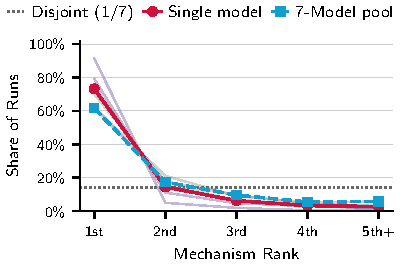
\includegraphics[width=\textwidth]{../figures/fig1_frontier_monoculture.pdf}
\caption{Share of runs on each scenario's 1st to 5th+ mechanisms across seven models (faint lines, solid mean). Pooling all seven models (dashed) still leaves 61.7\% of runs on the most common mechanism, compared to at most 14.3\% if the seven models never overlapped (dotted).}
\label{fig:frontier}
\end{minipage}\hfill
\begin{minipage}[t]{0.48\textwidth}
\centering
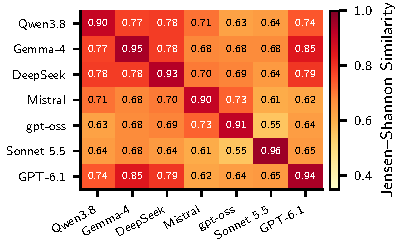
\includegraphics[width=\textwidth]{../figures/fig2_hivemind_heatmap.pdf}
\caption{Jensen--Shannon similarity of mechanism distributions across seven models ($n=15$ runs per half). Diagonal cells compare two halves of the same model's runs (mean 0.93), and off-diagonal cells compare different models (mean 0.69 vs.\ 0.37 if models favored unrelated mechanisms).}
\label{fig:hivemind}
\end{minipage}
\end{figure}

\textbf{High similarity across models.} Different models favor largely the same explanations. Jensen--Shannon similarity across model pairs averages 0.69. That is lower than when comparing two halves of the same model's runs, showing that models are not identical, yet far higher than if each model favored unrelated mechanisms (Figure~\ref{fig:hivemind}). Pairs of models select the same modal mechanism in more than half of comparisons, and pooling all seven models still leaves 62\% of runs on one shared mechanism (Figure~\ref{fig:frontier}). Sampling equally across all seven models exceeds the single-model mean on $\mathrm{TED}$, yet remains slightly below the highest-scoring individual model (Appendix Table~\ref{tab:frontier}). \citet{vanderschaar2026creativity} propose that a system of several agents provides alternative formulations because the agents differ. Our seven models from six laboratories propose largely the same causal mechanisms. Two tightly constrained clinical cases converge on essentially one mechanism across all models, yet single-model monoculture remains near or above 50\% even on open-ended scenarios where the seven models collectively uncover up to ten valid mechanisms.

\subsection{Experiment 2. Post-Training and Scale in \texttt{OLMo-3}}

\textbf{Reasoning distillation drives monoculture.} We evaluate 12 open \texttt{OLMo-3} checkpoints \citep{olmo2025olmo3} spanning pretrained 7B and 32B base models (raw completion), \texttt{7B-Instruct}, \texttt{7B-Think}, and matched \texttt{32B-Think} across SFT, DPO, and RLVR, plus \texttt{OLMo-3.1-32B-Think} (Figure~\ref{fig:olmo}, Appendix Table~\ref{tab:olmo}). Comparing checkpoints on valid runs at equal sample size ($\mathrm{SMR}_{\mathrm{val}@5}$) reveals three patterns. First, supervised instruction tuning from the 7B base model raises validity without increasing monoculture among valid runs, whereas distilling reasoning traces at 7B SFT causes the largest statistically significant increase in monoculture (58\% to 79\%). On the 7B instruction line, RLVR raises raw $\mathrm{SMR}$ significantly with a smaller, non-significant increase among valid runs. Second, DPO and RLVR leave monoculture statistically flat on both the 7B and 32B reasoning lines, while still improving validity at 7B. Third, scaling the reasoning recipe from 7B to 32B raises $\mathrm{TVR}$ substantially (66\% to 93\% at SFT) without increasing monoculture.

\begin{figure}[t]
\centering
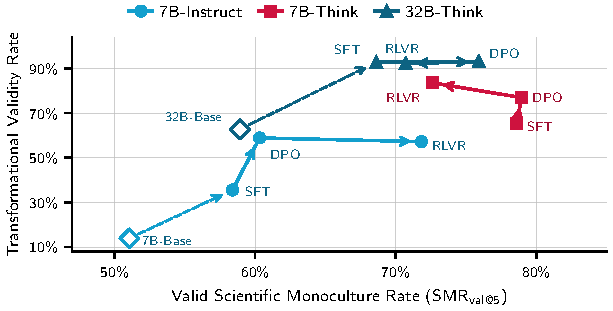
\includegraphics{../figures/fig3_olmo_posttraining.pdf}
\caption{Monoculture among valid outputs at equal sample size ($\mathrm{SMR}_{\mathrm{val}@5}$) versus validity ($\mathrm{TVR}$) across matched \texttt{OLMo-3} checkpoints. Distilling reasoning traces at 7B SFT shifts monoculture from 58\% to 79\%, whereas subsequent DPO and RLVR leave monoculture flat on reasoning lines and scaling from 7B to 32B raises validity without increasing monoculture.}
\label{fig:olmo}
\end{figure}

\subsection{Experiment 3. Inference-Time Interventions and Prompt-Resistant Mode Collapse}

We compare four inference-time methods against Baseline on all five open-weight models. On both proprietary models we run every method except High-Temperature Sampling, because their APIs fix sampling temperature at $T=1.0$. Each method produces $N=30$ runs per scenario (Figure~\ref{fig:pareto}, Appendix Table~\ref{tab:interv}, prompts in Appendix~\ref{app:prompts}).
\begin{itemize}[leftmargin=1.5em, itemsep=0pt, topsep=1pt]
\item \textbf{High-Temperature Sampling} raises sampling temperature from $T=1.0$ to $T=1.3$.
\item \textbf{In-Context Regeneration (ICR)}, adapted from TwistBench, runs three 10-turn chains forbidding prior hypotheses.
\item \textbf{Verbalized Sampling (VS)} \citep{zhang2025verbalized} requests five distinct hypotheses with estimated probabilities in one call (six calls per scenario).
\item \textbf{Two-Stage Axiom-Negation} extracts six implicit assumptions of the prevailing theory, then prompts the model to drop each assumption in turn for five runs.
\end{itemize}

\textbf{High-Temperature Sampling fails.} Raising temperature to $T=1.3$ does not significantly reduce $\mathrm{SMR}$ on four of five open-weight models while significantly reducing $\mathrm{TVR}$ on \texttt{Qwen3.8} and \texttt{Mistral-3.5} (Appendix Table~\ref{tab:interv}). On \texttt{DeepSeek-V4}, a modest $\mathrm{SMR}$ decrease is accompanied by a reduction in $\mathrm{TVR}$ to 49\%.

\begin{figure}[t]
\centering
\begin{minipage}[t]{0.48\textwidth}
\centering
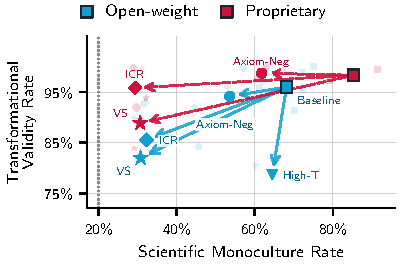
\includegraphics[width=\textwidth]{../figures/fig4_interventions_pareto.pdf}
\caption{Mean shifts in $\mathrm{SMR}$ and $\mathrm{TVR}$ from Baseline (squares) across 12 scenarios for five open-weight models (cyan) and two proprietary models (crimson). Dotted line marks the 20\% floor of 5-item VS.}
\label{fig:pareto}
\end{minipage}\hfill
\begin{minipage}[t]{0.48\textwidth}
\centering
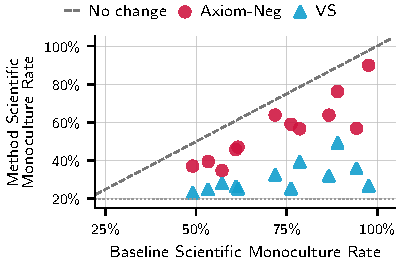
\includegraphics[width=\textwidth]{../figures/fig5_attractor_reconvergence.pdf}
\caption{Per-scenario $\mathrm{SMR}$ (mean across all seven models) under Baseline versus Axiom-Negation and VS across all 12 anomalies. Axiom-Negation remains well above VS, which clusters near the 20\% dotted floor.}
\label{fig:attractor}
\end{minipage}
\end{figure}

\textbf{Axiom-Negation yields partial or null gains.} Prompting models to drop six distinct implicit assumptions does not significantly reduce $\mathrm{SMR}$ on \texttt{Qwen3.8-27B} or \texttt{Gemma-4-31B} (Appendix Table~\ref{tab:interv}). It produces only a partial reduction on the other five models, leaving 45\% to 68\% $\mathrm{SMR}$ across all seven models and remaining far above VS and ICR across scenarios (Figure~\ref{fig:attractor}). Models often map different negated assumptions back to their default explanation even on open-ended cases. For instance, \texttt{GPT-6.1 Terra} returns to its most common Baseline mechanism on \texttt{clin\_01} (circadian dosing alignment) in 23 of 30 Axiom-Negation runs versus 22 of 30 under Baseline.

\textbf{Verbalized Sampling and ICR.} Both Verbalized Sampling and In-Context Regeneration significantly reduce $\mathrm{SMR}$ on all seven open-weight and proprietary models, lowering it to 29\% to 38\% (Appendix Table~\ref{tab:interv}). Under VS, two factors account for $\mathrm{SMR}$ remaining near 30\%. First, requesting five hypotheses per call imposes a 20\% lower bound whenever each call includes the model's default mechanism once. Second, at least two of the five hypotheses are still assigned to the same mechanism in 42\% to 71\% of calls. VS also lowers $\mathrm{TVR}$ significantly on five models, particularly \texttt{Mistral-3.5} and \texttt{gpt-oss-120b}. VS responses are roughly one-quarter to three-fifths the length of Baseline responses and score slightly lower on all three axes, so part of this validity reduction likely stems from generating five shorter hypotheses within a single response. In-Context Regeneration generates one full hypothesis per turn and achieves higher $\mathrm{TED}$ than VS on five of seven models, including both proprietary models (\texttt{Claude Sonnet 5.5} reaches $\mathrm{TED}=5.70$ at nearly 100\% validity).

\subsection{Experiment 4. Memorization Controls on Historical vs.\ Transferred Cases}

\textbf{Historical vs.\ transferred cases.} We run Baseline on the four memorization controls from Section~\ref{sec:benchmark} with all five open-weight models (Figure~\ref{fig:contam}, Appendix Table~\ref{tab:frontier}). Mean $\mathrm{SMR}$ falls from 84\% on historical cases to 65\% on transferred cases and is lower on transferred cases for all five models. Mean $\mathrm{TVR}$ shifts from 99\% to 94\%. Monoculture nevertheless remains at 65\% on the newly written transferred cases, so memorization does not explain it. This comparison is descriptive because it rests on four scenario pairs.

\begin{figure}[t]
\centering
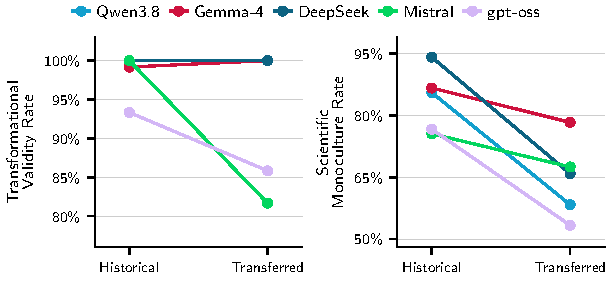
\includegraphics{../figures/fig6_contamination_controls.pdf}
\caption{Experiment 4 memorization controls across four historical cases and their transferred cases. Every open-weight model shows lower $\mathrm{SMR}$ on transferred cases, while $\mathrm{TVR}$ drops on \texttt{Mistral-3.5} and \texttt{gpt-oss-120b}.}
\label{fig:contam}
\end{figure}

\section{Related Work}
\label{sec:related}

Our framing builds on \citet{boden2004creative}, \citet{kuhn1962structure}, and \citet{vanderschaar2026creativity}, alongside \citet{vanderschaar2026openbeginningness} on formulating problems from raw phenomena. We extend TwistBench \citep{schapiro2026twistbench} from literary plot twists to scientific anomalies, a direction its authors propose as future work. TwistBench already reports mode collapse among high-quality twists. It treats a requested twist as transformational creativity. Under the stricter definition of \citet{vanderschaar2026creativity}, a requested reframing does not count because the system does not initiate it. The validity near 100\% that we observe suggests that benchmarks of this kind measure compliance and diversity rather than the capacity to initiate a revision. NoveltyBench \citep{zhang2025noveltybench} groups open-ended responses into functional equivalence classes, whereas we cluster hypotheses by causal mechanism under explicit experimental constraints. Prior work shows that post-training and model scale can narrow output diversity \citep{kirk2024understanding,zhang2025noveltybench}. Reduced diversity has also been reported when people write with language models \citep{padmakumar2024does}. It raises concerns about scientific monoculture as language models are used for research ideation \citep{si2024can,lu2024aiscientist,traberg2026monoculture}. In our \texttt{OLMo-3} results, monoculture among valid hypotheses increases at reasoning distillation. It does not increase at later preference and reinforcement stages or at larger scale. Finally, we adapt Verbalized Sampling \citep{zhang2025verbalized} and Vendi Scores \citep{friedman2023vendi} to hypothesis generation.

\section{Limitations}
\label{sec:limitations}

Three limitations qualify our findings. First, all 12 scenarios were written with a single LLM, and some tightly constrained cases admit essentially one canonical explanation, so part of measured monoculture comes from the scenarios themselves. Second, our evaluation relies on LLM judges reading text alone. Judge pairs show only moderate weighted $\kappa$ (0.19 to 0.65), and differences in judge strictness shift absolute $\mathrm{TVR}$ levels even though model rankings remain nearly unchanged. In addition, Baseline $\mathrm{TVR}$ approaches 100\% on strong models. Third, our prompts request the reframing explicitly, so we do not test whether models initiate a revision unprompted.

\section{What I Would Do With More Time}
\label{sec:future}

\textbf{Use real anomalies and human domain experts.} Evaluating models on real experimental anomalies published after training cutoffs, scored blindly by domain scientists, would show how much monoculture comes from the models rather than from anomalies that admit a single plausible explanation. Expert ratings would also test scientific realism without relying solely on LLM judges.

\textbf{Test hypotheses with domain simulators.} Pairing each scenario with a runnable simulator would allow us to test directly whether a proposed mechanism reproduces the anomalous data.

\textbf{Locate and train against monoculture.} Verbalized Sampling shows that models can produce causal mechanisms that Baseline rarely reaches. Comparing internal activations under Baseline and Verbalized Sampling could test whether the dominant causal mechanism is fixed before generation begins or emerges during it. Fine-tuning one base model with a reward for valid diversity across causal mechanisms would test directly whether post-training causes monoculture and whether it can be mitigated during training.

\section{Use of AI Tools}
\label{sec:ai}

Claude Code was used for coding, running experiments, and generating plots. Gemini 4 Neon was used to generate the benchmark scenarios, prompt templates, and judge calibration set, and to assist with manuscript editing.

\clearpage
\bibliography{references}
\bibliographystyle{iclr2026_conference}

\clearpage
\appendix
\section{Full Quantitative Results}
\label{app:tables}

\noindent\textbf{Metric Glossary}
\begin{itemize}[leftmargin=1.5em, itemsep=1pt, topsep=3pt]
\item $S$, $C$, $R$ are mean 1--5 ratings for Surprise, Empirical Coherence, and Scientific Realism across three or four judges from other model families.
\item $\mathrm{TVR}$ is Transformational Validity Rate, and $\mathrm{CCR}$ is Constraint Contradiction Rate (the share of hypotheses where at least half of the judges mark at least one constraint as contradicted).
\item $\mathrm{SMR}$, $\mathrm{SMR}_{\mathrm{val}}$, and $\mathrm{SMR}_{\mathrm{val}@5}$ are Scientific Monoculture Rate (share of the single most frequent named mechanism, excluding non-explanatory outputs and never counting the miscellaneous catch-all category as a repeated mechanism) across all runs, across valid runs only, and across subsamples of 5 valid runs per scenario ($n/12$ scenarios with at least 5 valid runs).
\item $N_{\mathrm{eff}}$ is the effective number of frameworks ($\exp H$), and $\mathrm{TED} = \mathrm{TVR}\cdot N_{\mathrm{eff}}(\mathcal{T})$ is Transformational Effective Diversity.
\item $\mathrm{Vendi}_{\mathrm{mech}}$ is the Vendi Score computed from \texttt{Qwen3-Embedding-0.6B} embeddings of the mechanism summaries.
\item Historical and Transferred $\mathrm{SMR}$ report Experiment 4 monoculture on the historical and transferred cases.
\item Stars mark two-sided paired Wilcoxon tests across 12 scenarios after Benjamini--Hochberg FDR correction ($^*q<0.05$, $^{**}q<0.01$).
\end{itemize}

\begin{table}[ht]
\centering
\caption{Experiment 1 Baseline results across five open-weight and two proprietary models (12 anomalies, $N=30$ runs each) and Experiment 4 memorization controls (4 historical and 4 transferred cases).}
\label{tab:frontier}
\resizebox{\textwidth}{!}{%
\begin{tabular}{lcccccccccc}
\toprule
Model & $S$ & $C$ & $R$ & TVR (\%) & SMR (\%) $\downarrow$ & $N_{\mathrm{eff}}$ $\uparrow$ & TED $\uparrow$ & $\mathrm{Vendi}_{\mathrm{mech}}$ & Historical SMR & Transferred SMR \\
\midrule
Qwen3.8-27B & \textbf{4.23} & 4.60 & \textbf{4.55} & 97.2 & 61.9 & \textbf{3.08} & \textbf{3.05} & \textbf{3.64} & 85.6 & 58.3 \\
Gemma-4-31B & 4.06 & 4.33 & 4.26 & \textbf{100.0} & 75.0 & 2.13 & 2.13 & 2.87 & 86.7 & 78.3 \\
DeepSeek-V4-Flash & 4.14 & 4.47 & 4.37 & 95.6 & 72.5 & 2.36 & 2.25 & 3.07 & 94.2 & 65.8 \\
Mistral-3.5-128B & 3.95 & 4.19 & 3.96 & 91.4 & 70.1 & 2.51 & 2.21 & 2.80 & 75.6 & 67.5 \\
gpt-oss-120b & 4.10 & \textbf{4.61} & 4.24 & 95.8 & \textbf{61.1} & 2.82 & 2.56 & 3.20 & 76.7 & 53.3 \\
\midrule
Claude Sonnet 5.5 & 4.13 & 4.50 & 4.45 & 99.4 & 91.4 & 1.46 & 1.44 & 2.52 & -- & -- \\
GPT-6.1 Terra & 4.00 & 4.60 & 4.50 & 97.2 & 79.2 & 2.02 & 1.97 & 2.62 & -- & -- \\
\midrule
5-Open Ensemble (6$\times$5) & -- & -- & -- & 96.1 & 60.6 & 3.17 & 2.99 & -- & -- & -- \\
7-Model Ensemble (4$\times$7) & -- & -- & -- & 97.6 & 61.8 & 3.10 & 2.99 & -- & -- & -- \\
\bottomrule
\end{tabular}}
\end{table}

\begin{table}[ht]
\centering
\caption{Experiment 2 results across 12 \texttt{OLMo-3} and \texttt{OLMo-3.1} checkpoints. Pretrained base models use raw completion, and all other checkpoints use the standard chat template. Stars ($^*q<0.05$, FDR-corrected) mark significant changes relative to each line's reference checkpoint (SFT vs.\ Base, DPO/RLVR vs.\ SFT, and \texttt{7B-Think-SFT} vs.\ \texttt{7B-Inst-SFT}).}
\label{tab:olmo}
\resizebox{\textwidth}{!}{%
\begin{tabular}{llcccccccc}
\toprule
Group & Checkpoint & TVR (\%) & CCR (\%) $\downarrow$ & SMR (\%) $\downarrow$ & $\mathrm{SMR}_{\mathrm{val}}$ & $\mathrm{SMR}_{\mathrm{val}@5}$ ($n$) & $N_{\mathrm{eff}}$ $\uparrow$ & TED $\uparrow$ & $\mathrm{Vendi}_{\mathrm{mech}}$ \\
\midrule
OLMo3 Base & 7B-Base & 13.9 & 46.9 & 38.2 & 59.9 & 51.1 (8) & 4.35 & 0.43 & 3.92 \\
 & 32B-Base & 62.8 & 16.4 & 43.9 & 51.9 & 58.9 (11) & 4.32 & 2.21 & 3.53 \\
\midrule
OLMo3-7B-Inst & SFT & 35.6$^*$ & 34.4 & 41.7 & 61.4 & 58.4 (10) & 4.34 & 1.18$^*$ & 3.88 \\
 & DPO & 58.9$^*$ & 22.2 & 53.0 & 53.5 & 60.3 (11) & 3.76 & 2.25 & 3.33 \\
 & RLVR & 57.2$^*$ & 20.0 & 62.6$^*$ & 68.6 & 71.8 (11) & 3.19 & 1.67 & 3.20 \\
\midrule
OLMo3-7B-Think & Think-SFT & 65.6$^*$ & 12.8 & 70.1$^*$ & 76.7 & 78.6$^*$ (11) & 2.57 & 1.32 & 2.98 \\
 & Think-DPO & 76.9$^*$ & 9.7 & 72.7 & 80.2 & 79.0 (11) & 2.47 & 1.61 & 2.96 \\
 & Think-RLVR & 83.6$^*$ & 6.7 & 69.3 & 69.7 & 72.6 (12) & 2.40 & 1.81 & 2.88 \\
\midrule
OLMo3-32B-Think & Think-SFT & 92.8$^*$ & 2.5 & 64.6$^*$ & 64.6 & 68.6 (12) & 3.06 & 2.67 & 2.99 \\
 & Think-DPO & 93.1 & 3.1 & 70.3 & 73.2 & 75.9 (12) & 2.56 & 2.16 & 2.95 \\
 & Think-RLVR & 92.2 & 2.8 & 68.4 & 67.9 & 70.7 (12) & 2.86 & 2.55 & 3.08 \\
OLMo3.1-32B & 32B-Think & \textbf{95.3} & \textbf{1.4} & 71.7 & 71.9 & 76.0 (12) & 2.51 & 2.28 & 2.95 \\
\bottomrule
\end{tabular}}
\end{table}

\begin{table}[ht]
\centering
\caption{Experiment 3 inference-time interventions across all five open-weight models and both proprietary models (12 anomalies, $N=30$ runs each). Stars mark significant changes relative to each model's Baseline after Benjamini--Hochberg FDR correction ($^*q<0.05$, $^{**}q<0.01$).}
\label{tab:interv}
\resizebox{\textwidth}{!}{%
\begin{tabular}{llccccccc}
\toprule
Model & Condition & TVR (\%) & CCR (\%) $\downarrow$ & SMR (\%) $\downarrow$ & $\mathrm{SMR}_{\mathrm{val}}$ & $N_{\mathrm{eff}}$ $\uparrow$ & TED $\uparrow$ & $\mathrm{Vendi}_{\mathrm{mech}}$ \\
\midrule
Qwen3.8-27B & Baseline ($T=1.0$) & 97.2 & 0.0 & 61.9 & 61.8 & 3.08 & 3.05 & 3.64 \\
 & High-Temp ($T=1.3$) & 80.3$^{**}$ & 0.6 & 60.2 & 60.8 & 3.12 & 2.42 & 3.93 \\
 & Axiom-Negation & 96.1 & 0.3 & 53.0 & 53.6 & 3.43 & 3.31 & 3.95 \\
 & In-Context Regen. & 86.4$^*$ & 1.1 & 37.7$^{**}$ & 41.5$^{**}$ & 4.88 & 4.22$^*$ & \textbf{4.73} \\
 & Verbalized Sampling & \textbf{99.7} & 0.0 & \textbf{31.1}$^{**}$ & \textbf{31.2}$^{**}$ & \textbf{5.56} & \textbf{5.50}$^{**}$ & 4.32 \\
\midrule
Gemma-4-31B & Baseline ($T=1.0$) & 100.0 & 0.0 & 75.0 & 75.0 & 2.13 & 2.13 & 2.87 \\
 & High-Temp ($T=1.3$) & 98.9 & 0.0 & 72.2 & 72.5 & 2.11 & 2.06 & 2.92 \\
 & Axiom-Negation & 98.9 & 0.0 & 67.5 & 67.6 & 2.31 & 2.27 & 2.98 \\
 & In-Context Regen. & 92.8$^*$ & 0.0 & 31.7$^{**}$ & \textbf{31.2}$^{**}$ & 5.07 & \textbf{4.79}$^{**}$ & \textbf{4.43} \\
 & Verbalized Sampling & 89.7$^{**}$ & 1.1 & \textbf{29.1}$^{**}$ & 32.0$^{**}$ & \textbf{5.46} & 4.77$^{**}$ & 4.17 \\
\midrule
DeepSeek-V4-Flash & Baseline ($T=1.0$) & 95.6 & 0.0 & 72.5 & 72.5 & 2.36 & 2.25 & 3.07 \\
 & High-Temp ($T=1.3$) & 49.4$^{**}$ & 1.1 & 60.5$^*$ & 64.2 & 3.02 & 1.21$^{**}$ & 3.69 \\
 & Axiom-Negation & \textbf{99.7} & 0.0 & 57.0$^*$ & 57.0$^*$ & 3.22 & 3.21$^*$ & 3.32 \\
 & In-Context Regen. & 88.6$^*$ & 2.2 & \textbf{30.3}$^{**}$ & \textbf{29.8}$^{**}$ & 5.37 & 4.70$^{**}$ & \textbf{4.94} \\
 & Verbalized Sampling & 93.6 & 3.3 & 32.1$^{**}$ & 33.8$^{**}$ & \textbf{5.53} & \textbf{5.12}$^{**}$ & 4.10 \\
\midrule
Mistral-3.5-128B & Baseline ($T=1.0$) & 91.4 & 2.2 & 70.1 & 71.7 & 2.51 & 2.21 & 2.80 \\
 & High-Temp ($T=1.3$) & 71.1$^{**}$ & 4.7 & 68.1 & 74.1 & 2.75 & 1.64 & 3.05 \\
 & Axiom-Negation & 84.2 & 4.7 & 45.7$^{**}$ & 51.6$^{**}$ & 3.96 & 3.11 & 3.35 \\
 & In-Context Regen. & 70.8$^*$ & 2.8 & \textbf{30.4}$^{**}$ & \textbf{36.3}$^{**}$ & 5.08 & \textbf{3.45} & 3.99 \\
 & Verbalized Sampling & 60.6$^{**}$ & 11.4 & 31.7$^{**}$ & 41.5$^{**}$ & \textbf{5.65} & 2.89 & \textbf{4.01} \\
\midrule
gpt-oss-120b & Baseline ($T=1.0$) & 95.8 & 0.8 & 61.1 & 62.9 & 2.82 & 2.56 & 3.20 \\
 & High-Temp ($T=1.3$) & 93.6 & 0.6 & 61.3 & 62.2 & 2.74 & 2.46 & 3.46 \\
 & Axiom-Negation & 91.9 & 4.7 & 44.6$^*$ & 46.1$^*$ & 3.90 & 3.50 & 3.69 \\
 & In-Context Regen. & 89.2$^*$ & 0.0 & 31.2$^{**}$ & \textbf{32.9}$^{**}$ & 5.12 & \textbf{4.66}$^{**}$ & 4.31 \\
 & Verbalized Sampling & 66.4$^{**}$ & 12.2 & \textbf{29.7}$^{**}$ & 37.0$^*$ & \textbf{5.55} & 3.24 & \textbf{4.38} \\
\midrule
Claude Sonnet 5.5 & Baseline ($T=1.0$) & 99.4 & 0.0 & 91.4 & 91.7 & 1.46 & 1.44 & 2.52 \\
 & Axiom-Negation & \textbf{100.0} & 0.0 & 63.0$^{**}$ & 63.0$^{**}$ & 2.73 & 2.73$^{**}$ & 3.07 \\
 & In-Context Regen. & 99.7 & 0.0 & \textbf{29.0}$^{**}$ & \textbf{29.1}$^{**}$ & \textbf{5.72} & \textbf{5.70}$^{**}$ & \textbf{4.59} \\
 & Verbalized Sampling & 93.9$^*$ & 1.9 & 32.2$^{**}$ & 34.0$^{**}$ & 5.58 & 5.04$^{**}$ & 4.13 \\
\midrule
GPT-6.1 Terra & Baseline ($T=1.0$) & 97.2 & 0.0 & 79.2 & 77.6 & 2.02 & 1.97 & 2.62 \\
 & Axiom-Negation & \textbf{97.5} & 0.0 & 60.5$^{**}$ & 60.5$^*$ & 2.87 & 2.78$^*$ & 3.21 \\
 & In-Context Regen. & 91.9 & 0.0 & 29.7$^{**}$ & 31.8$^{**}$ & 5.50 & \textbf{5.03}$^{**}$ & \textbf{4.67} \\
 & Verbalized Sampling & 83.9$^{**}$ & 0.3 & \textbf{29.1}$^{**}$ & \textbf{29.3}$^{**}$ & \textbf{5.55} & 4.44$^{**}$ & 3.98 \\
\bottomrule
\end{tabular}}
\end{table}

\clearpage
\section{Sci-TwistBench Scenarios}
\label{app:scenarios}

Table~\ref{tab:scenarios_overview} lists all 12 core scenarios across the four disciplines. Below it, we reproduce one complete scenario and its four explicit experimental constraints ($E_1$--$E_4$) from each discipline verbatim.

\begin{table}[h]
\centering
\caption{Overview of the 12 synthetic scientific anomaly scenarios in Sci-TwistBench.}
\label{tab:scenarios_overview}
\small
\setlength{\tabcolsep}{5.0pt}
\begin{tabular}{llp{4.8cm}p{5.0cm}}
\toprule
ID & Domain & Scenario Title & Prevailing Theory \\
\midrule
\texttt{clin\_01} & Clinical & Bimodal Center Efficacy in a Lipid Trial & Efficacy scales monotonically with steady-state plasma drug exposure (AUC). \\
\texttt{clin\_02} & Clinical & Rapid-Clearance Mortality in Septic Shock & Faster bactericidal clearance monotonically improves host survival. \\
\texttt{clin\_03} & Clinical & Non-Monotonic Motor Recovery After Stroke & Residual corticospinal tract integrity is monotonically beneficial for recovery. \\
\texttt{phys\_01} & Physics & Thickness-Inverted Thermal Conductivity & Thinner dielectric films strictly lower thermal conductivity via boundary scattering. \\
\texttt{phys\_02} & Physics & Annual Drift Between Optical Lattice Clocks & Static elevation and local gravimetry remove environmental redshift drift. \\
\texttt{phys\_03} & Physics & Capacity Gain Under Open-Circuit Rest & Cycle-1 capacity is maximal and resting causes only monotonic calendar fade. \\
\texttt{ecol\_01} & Ecology & Predator-Exclusion Herbivore Collapse & Removing apex predators monotonically increases herbivore biomass. \\
\texttt{ecol\_02} & Ecology & Boreal Carbon-Sink Surge Amid Drought & Severe drought reduces boreal carbon uptake in proportion to canopy decline. \\
\texttt{ecol\_03} & Ecology & Daytime Urban Cooling in Extreme Heatwaves & Impervious urban surfaces monotonically amplify daytime heatwave warmth. \\
\texttt{econ\_01} & Economics & Market Contraction Under Price Transparency & Public price benchmarks reduce friction and increase match volume. \\
\texttt{econ\_02} & Economics & Accuracy Collapse Under Auditing Bonuses & Proper accuracy bonuses improve detection of subtle statistical errors. \\
\texttt{econ\_03} & Economics & Commute Expansion After Express Rail Launch & Faster transit lowers door-to-door commutes when highway speeds also rise. \\
\bottomrule
\end{tabular}
\end{table}

\begin{scenariobox}{Example 1 (\texttt{clin\_01}, Clinical and Biomedical)}
A multi-center, double-blind, placebo-controlled Phase-III clinical trial ($N = 1,840$ across 14 academic hospitals) evaluated KVX-402, an oral selective hepatic enzyme inhibitor designed to lower serum LDL cholesterol in patients with refractory hyperlipidemia. Under the prevailing pharmacokinetic paradigm, LDL reduction should scale monotonically with 24-hour steady-state systemic plasma exposure (AUC) of the parent compound, independent of treatment center logistics. Across the pooled cohort, KVX-402 produced only a modest mean LDL reduction of $-9.4\%$ relative to placebo ($p = 0.04$).

Pre-specified site-level auditing uncovered a striking bimodal divergence that completely explains the weak pooled effect. At 5 hospitals (Group A, $n = 660$), KVX-402 achieved a dramatic $-34.2\%$ LDL reduction ($p < 10^{-9}$), whereas at the other 9 hospitals (Group B, $n = 1,180$), treated patients exhibited a slight numerical worsening of $+4.1\%$ ($p = 0.08$). Blinded central LC-MS/MS assays verified identical active-ingredient purity, tablet stability, and 24-hour systemic plasma AUC of KVX-402 across all 14 hospitals (mean AUC ratio Group A/B $= 1.02$, $p = 0.71$). Baseline patient genetics (APOE and PCSK9 variants), age, BMI, statin background, and standardized 7-day dietary logs were statistically indistinguishable between Group A and Group B (all $p > 0.40$).

To test whether unmeasured patient-level confounders drove the split, 64 non-responding patients from Group B hospitals were transferred into a 6-week open-label crossover protocol managed at Group A hospitals using the exact same drug lot numbers. Their LDL dropped by a mean of $-31.8\%$ ($p < 10^{-8}$). Placebo-arm patients showed virtually zero LDL change in both Group A ($-0.3\% \pm 1.1\%$) and Group B ($+0.2\% \pm 1.2\%$), ruling out generic hospital care or diet effects.

\textbf{Hard constraints.}
($E_1$) Blinded LC-MS/MS confirms identical pill purity and 24-hour systemic plasma AUC across Group A and Group B ($p = 0.71$).
($E_2$) Baseline genetics, age, BMI, statin use, and dietary logs are matched across groups (all $p > 0.40$).
($E_3$) Transferring 64 Group B non-responders to Group A hospitals using identical drug lots restores $-31.8\%$ LDL reduction within 6 weeks.
($E_4$) Placebo arms show zero LDL change in both groups, proving the center factor interacts specifically with KVX-402.
\end{scenariobox}

\begin{scenariobox}{Example 2 (\texttt{phys\_01}, Physics and Materials)}
A materials physics collaboration measured the cross-plane and in-plane thermal conductivity ($\kappa_{\mathrm{eff}}$) of epitaxial layered perovskite-oxide thin films ($\mathrm{Sr_2TiO_4}$ grown on single-crystal MgO substrates) across thicknesses $d$ ranging from 20 nm to 800 nm at 300 K using time-domain thermoreflectance (TDTR). Standard kinetic theory of dielectric solids predicts that phonon-boundary scattering should reduce $\kappa_{\mathrm{eff}}$ monotonically below the bulk single-crystal value ($5.6\ \mathrm{W/m\cdot K}$) as film thickness decreases into the Casimir regime.

While films between 200 nm and 800 nm behaved normally ($\kappa_{\mathrm{eff}}$ dropping from 5.3 to $4.4\ \mathrm{W/m\cdot K}$), films thinner than 120 nm exhibited a dramatic inversion. At $d = 35$ nm, $\kappa_{\mathrm{eff}}$ surged to $18.4\ \mathrm{W/m\cdot K}$, more than triple the bulk single-crystal limit. Cross-sectional STEM and X-ray diffraction confirmed exact stoichiometry, single-phase crystallinity, and electrical resistivity exceeding $10^{11}\ \Omega\cdot\mathrm{cm}$ at all thicknesses, ruling out metallic inclusions or electronic heat conduction. Independent contact $3\omega$ electrical thermometry reproduced the $18.4\ \mathrm{W/m\cdot K}$ value within 4\%, ruling out optical penetration-depth artifacts specific to TDTR.

Substrate-exchange experiments isolated a sharp boundary condition. Growing the identical 35 nm $\mathrm{Sr_2TiO_4}$ film on compressive $\mathrm{LaAlO_3}$ eliminated the enhancement ($\kappa_{\mathrm{eff}} = 4.1\ \mathrm{W/m\cdot K}$), and mechanically exfoliating and transferring the 35 nm film off MgO onto amorphous $\mathrm{SiO_2}$ caused $\kappa_{\mathrm{eff}}$ to collapse immediately from 18.4 to $4.3\ \mathrm{W/m\cdot K}$. Moreover, when the intact 35 nm film on MgO was cooled to 80 K, the anomalous enhancement vanished completely and $\kappa_{\mathrm{eff}}$ reverted to normal Casimir scaling.

\textbf{Hard constraints.}
($E_1$) STEM/XRD confirm pure stoichiometry and resistivity $> 10^{11}\ \Omega\cdot\mathrm{cm}$, ruling out electronic conduction or metallic phases.
($E_2$) Optical TDTR and contact $3\omega$ thermometry agree within 4\%, ruling out optical transparency artifacts.
($E_3$) The 35 nm enhancement occurs on tensile MgO, vanishes on compressive $\mathrm{LaAlO_3}$ ($4.1\ \mathrm{W/m\cdot K}$), and vanishes when exfoliated onto $\mathrm{SiO_2}$ ($4.3\ \mathrm{W/m\cdot K}$).
($E_4$) Cooling the intact 35 nm film on MgO to 80 K eliminates the enhancement completely, restoring normal Casimir scaling.
\end{scenariobox}

\begin{scenariobox}{Example 3 (\texttt{ecol\_01}, Ecology and Earth Systems)}
A 5-year controlled marine-ecology field experiment across 36 coastal rocky-reef plots ($500\ \mathrm{m}^2$ each) tested classic top-down trophic cascade theory by excluding apex predatory crabs and wrasses using large-mesh cages to allow herbivorous purple sea urchins to proliferate. Standard trophic theory predicts that predator removal should sharply increase urchin biomass and intensify grazing until kelp forests collapse into urchin barrens.

During months 1 through 4, exclusion plots followed textbook predictions, with juvenile urchin settlement and density reaching 2.1 times that of unfenced controls ($p < 10^{-5}$). Beginning in month 7, however, urchin populations inside exclusion plots crashed catastrophically. By month 18, total urchin biomass in predator-exclusion plots was 68\% lower than in control plots ($p < 10^{-8}$), and canopy kelp cover expanded by $+41\%$ relative to controls, the exact inverse of a standard trophic cascade.

Continuous underwater video and cage-integrity inspections confirmed zero apex predator intrusion or human harvesting, and in-situ loggers recorded identical water temperature, dissolved oxygen, salinity, and dissolved inorganic nitrogen fluxes across exclusion and control plots (all $p > 0.65$). Dead urchin tests collected during the months 7--14 die-off exhibited completely intact spines with zero mechanical bite marks, while surviving urchins in exclusion plots displayed severely elevated cellular heat-shock and metabolic stress markers and 55\% smaller gonad indices despite abundant standing kelp.

\textbf{Hard constraints.}
($E_1$) Verified mesh integrity and underwater video confirm zero apex predator intrusion or human harvesting.
($E_2$) Loggers confirm identical temperature, dissolved oxygen, salinity, and nutrient influx across plots (all $p > 0.65$).
($E_3$) Juvenile settlement surged $2.1\times$ during months 1--4 before crashing from month 7 onward to $-68\%$ biomass and $+41\%$ kelp cover.
($E_4$) Dead urchin tests had intact spines with zero bite marks, while surviving exclusion-plot urchins showed high metabolic stress and stunted gonads despite abundant kelp.
\end{scenariobox}

\begin{scenariobox}{Example 4 (\texttt{econ\_01}, Economics and Behavioral)}
An online skilled-freelance labor marketplace ran a 6-month cluster-randomized experiment across 24 non-overlapping skill categories ($N = 48,000$ active freelancers and $N = 190,000$ client job postings). In 12 treatment categories, the platform deployed an AI market-rate estimator that displayed the predicted median winning bid to both clients and freelancers prior to proposal submission. Standard search-and-matching economics predicts that reducing price uncertainty should narrow bid dispersion, speed up bargaining, and increase total matched transaction volume.

Bid dispersion indeed tightened by 47\% in treatment categories, and freelancer time-to-submit proposals fell by 38\%, ruling out interface friction or cognitive overload. Yet total completed match rates collapsed by 19.3\% relative to untreated control categories ($p < 10^{-12}$), average winning bids rose by 11.8\%, and top-decile freelancers (ranked by historical client ratings and repeat hires) exited the platform at 3.2 times the control attrition rate. Control categories remained completely flat throughout the 6 months, ruling out cross-market spillovers or macro shocks.

Subgroup decomposition revealed a stark task-structure interaction. Client posting volume and stated budgets did not drop during months 1--2 ($p = 0.44$), yet the match-rate decline began immediately in week 2. The collapse was concentrated almost entirely in complex, high-variance custom projects ($-31.4\%$ match rate), whereas standardized, commoditized tasks experienced a modest increase in match volume ($+4.2\%$, $p = 0.01$).

\textbf{Hard constraints.}
($E_1$) Cluster randomization across 24 non-overlapping categories confirms zero cross-market spillover and flat control match rates.
($E_2$) Client posting volume and budgets stayed flat in months 1--2 ($p = 0.44$), yet match rates dropped starting in week 2.
($E_3$) Match collapse occurred almost exclusively on complex projects ($-31.4\%$), while standardized tasks rose ($+4.2\%$), with $+11.8\%$ winning bids and $3.2\times$ top-decile exit.
($E_4$) Bid dispersion fell 47\% and submission time fell 38\%, ruling out interface friction or cognitive overload.
\end{scenariobox}

\subsection*{Memorization Control Pairs (Historical vs.\ Transferred)}

Table~\ref{tab:contam_overview} summarizes the four memorization controls used in Experiment 4, followed by one complete matched pair (\texttt{contam\_01}).

\begin{table}[ht]
\centering
\caption{Overview of the four memorization controls.}
\label{tab:contam_overview}
\resizebox{\textwidth}{!}{%
\begin{tabular}{lp{3.9cm}p{4.1cm}p{3.9cm}}
\toprule
Pair ID & Historical Case & Transferred Case & Shared Underlying Mechanism \\
\midrule
\texttt{contam\_01} & Peptic ulcer relapse (\textit{H.\ pylori}) & High-salinity desalination membrane pitting & Extremophilic microbe sheltered beneath barrier layer \\
\texttt{contam\_02} & Asymmetric maternity ward mortality (Semmelweis) & Asymmetric semiconductor wafer bay defects & Upstream vector contamination carried by staff \\
\texttt{contam\_03} & Antarctic ozone TOMS satellite vs.\ ground gap & Abyssal hydrothermal cabled-array vs.\ glider gap & Automated QC threshold filtering out extreme regime \\
\texttt{contam\_04} & Combat damage clustering on returning bombers (Wald) & Hail damage clustering on returned alpine drones & Survivorship bias inverting fatal impact locations \\
\bottomrule
\end{tabular}}
\end{table}

\begin{scenariobox}{Control Pair 1A (\texttt{contam\_01\_orig}, Historical Case)}
For decades, gastroenterology held that chronic peptic ulcers were caused purely by excess gastric acid, stress, and mucosal barrier breakdown, because the highly acidic stomach lumen (pH 1.5--2.0) was assumed to be a sterile environment hostile to microbial colonization. Potent H2-receptor antagonists reliably suppressed gastric acid secretion and healed over 85\% of duodenal ulcers on endoscopy within 8 weeks.

However, longitudinal follow-up across multiple hospital cohorts revealed a striking paradox. Within 12 months of stopping acid-suppressing drugs, over 75\% of patients suffered complete ulcer relapse, even when lifestyle, diet, and psychological stress markers remained stable. By contrast, a small clinic testing an older bismuth subcitrate regimen combined with short-course metronidazole achieved similar initial healing but recorded a 12-month relapse rate below 15\%, despite far weaker acid suppression.

Histological biopsies of ulcer margins routinely noted curved, spiral structures beneath the gastric mucus layer, which standard pathology dismissed as incidental post-biopsy contaminants or inert debris because conventional 48-hour aerobic plate cultures grew nothing.

\textbf{Hard constraints.}
($E_1$) Acid-suppressing H2 blockers heal $>85\%$ acutely yet $>75\%$ relapse within 12 months.
($E_2$) Bismuth plus metronidazole suppresses acid far less yet cuts 12-month relapse below 15\%.
($E_3$) Stomach pH is 1.5--2.0 and standard 48-hour aerobic cultures grow nothing.
($E_4$) Biopsies repeatedly show curved spiral structures beneath the mucus layer at ulcer margins.
\end{scenariobox}

\begin{scenariobox}{Control Pair 1B (\texttt{contam\_01\_iso}, Transferred Case)}
In industrial brine-concentration engineering, recurrent pitting corrosion of polyamide reverse-osmosis membranes operating in hyper-saline, high-chlorine feedwater (salinity 180 g/L, free chlorine 4.5 ppm) has long been attributed strictly to chemical oxidative stress and mechanical pressure cycling, because the extreme osmotic and oxidizing brine stream is considered completely abiotic. Dosing chemical anti-oxidant neutralizers halts active pit growth and restores 88\% of baseline flux recovery within 6 weeks.

Yet plant-level longitudinal audits uncovered a sharp anomaly. Within 9 months of returning membranes to normal operating buffer, 78\% of chemically restored modules suffered rapid recurrence of deep pitting at identical membrane zones despite stable pressure and feed chemistry. Conversely, an experimental facility flushing modules briefly with a weak non-oxidizing copper-thiazole biocide achieved slower initial flux restoration but slashed 9-month pitting recurrence below 14\%, despite providing zero chemical antioxidant protection.

Scanning electron microscopy of pit floors consistently revealed filamentous micro-nodules nestled beneath the polysaccharide-like scaling boundary layer, which engineers routinely dismissed as precipitated gypsum crystals because standard 48-hour freshwater nutrient-agar assays yielded zero colony growth.

\textbf{Hard constraints.}
($E_1$) Chemical antioxidant neutralizers restore 88\% flux acutely yet 78\% of modules relapse within 9 months.
($E_2$) Copper-thiazole biocide provides zero antioxidant protection yet cuts 9-month recurrence below 14\%.
($E_3$) Bulk brine is 180 g/L salinity with 4.5 ppm chlorine, and standard 48-hour freshwater agar shows zero growth.
($E_4$) SEM consistently reveals filamentous micro-nodules sheltered beneath the scaling boundary layer on pit floors.
\end{scenariobox}

\clearpage
\section{Prompt Templates and Evaluation Rubric}
\label{app:prompts}

All generation prompts share the same system instruction asking the model to act as an independent research scientist responding directly with mechanistically grounded reasoning. Below we show the user prompt templates for each condition and the judge rubric inside shaded prompt blocks.

\begin{promptbox}{Baseline and High-Temperature Generation}
Read the empirical summary below describing an unexplained scientific anomaly, then propose ONE concrete, paradigm-shifting scientific hypothesis that forces a re-interpretation of the prior observations while remaining strictly consistent with EVERY reported empirical finding and control measurement above. Avoid trivial explanations already ruled out by the controls, and avoid unphysical or unfalsifiable speculation. Format your response under four headings, namely Assumption Challenged (1--2 sentences), Core Hypothesis and Mechanism (1 concise paragraph), Reconciliation with Reported Data (2--4 bullet points), and Falsifiable Prediction (1--2 sentences specifying a discriminating test).
\end{promptbox}

\begin{promptbox}{Verbalized Sampling (VS)}
Rather than giving only the single most obvious explanation, survey the full space of genuinely distinct explanatory paradigms. Generate 5 FUNDAMENTALLY DIFFERENT paradigm-shifting scientific hypotheses for this anomaly. Each of the 5 hypotheses must challenge a DIFFERENT underlying assumption and propose a qualitatively distinct causal mechanism, not minor wording variants of the same idea, while remaining strictly consistent with EVERY reported empirical finding and control measurement above. For each hypothesis, estimate its relative prior plausibility probability between 0.01 and 0.99, including both high-probability and creative lower-probability tail hypotheses, and return a JSON array containing index, probability, assumption challenged, mechanism, reconciliation, and falsifiable prediction.
\end{promptbox}

\begin{promptbox}{In-Context Regeneration (ICR)}
Given the empirical summary and a bulleted list of all previously proposed explanatory frameworks in the current 10-turn chain (marked DO NOT REUSE, PARAPHRASE, OR VARIANT-MODIFY ANY OF THESE), propose ONE NEW, fundamentally distinct paradigm-shifting scientific hypothesis that explores a completely different causal mechanism and challenges a different underlying assumption than all prior frameworks while remaining strictly consistent with every reported finding and control measurement. Use the same four headings as Baseline generation.
\end{promptbox}

\begin{promptbox}{Two-Stage Axiom-Negation}
\textbf{Stage 1 (Assumption Audit).} Before proposing any explanations, perform a structural audit of the prevailing paradigm and identify exactly 6 distinct implicit assumptions spanning different axes (measurement or construct definition, causal direction or confounding, hidden system feedbacks, spatiotemporal or kinetic scales, population or selection structure, and boundary or environmental couplings). Return a JSON list of 6 assumptions with a negation direction for each.

\textbf{Stage 2 (Targeted Reframing).} Explicitly DROP or INVERT one targeted assumption from Stage 1 along its specified reframing direction. Constructing strictly from the negation or inversion of this specific assumption, develop ONE concrete, scientifically realistic, paradigm-shifting hypothesis that resolves the anomaly while remaining strictly consistent with every reported finding and control measurement. Use the same four headings as Baseline generation.
\end{promptbox}

\begin{promptbox}{Judge Rubric and Blind Taxonomy}
Each LLM judge receives the scenario text, its four hard constraints ($E_1$--$E_4$), and one candidate hypothesis, and returns a single JSON object containing five fields.
(1) \textbf{Constraint Audit}, labeling each of $E_1$--$E_4$ as CONSISTENT, PARTIAL, or CONTRADICTED.
(2) \textbf{Surprise and Reframing Depth (1--5)}, from 1 (trivial restatement or incoherent) and 2 (incremental tweak inside the prevailing theory) through 3 (combinatorial blend) to 4 (explicitly drops or inverts a core implicit assumption) and 5 (deep reframing under which all paradoxical facts cohere).
(3) \textbf{Empirical Coherence (1--5)}, strictly capped at 2 whenever any constraint $E_1$--$E_4$ is labeled CONTRADICTED, up to 5 (quantitatively reconciles all four constraints).
(4) \textbf{Scientific Realism and Falsifiability (1--5)}, from 1 (violates physical or biological laws) to 5 (domain-expert realism with a sharp discriminating test).
(5) \textbf{Canonical Extraction}, producing a 5--12 word assumption-dropped phrase and a neutral 15--28 word mechanism summary used to construct blinded causal taxonomies per scenario.
A hypothesis counts toward $\mathrm{TVR}$ if its mean judge ratings satisfy $S \ge 3.5$, $C \ge 3.5$, and $R \ge 3.5$ with zero majority-voted constraint contradictions.
\end{promptbox}

\clearpage
\section{Judge Calibration Set}
\label{app:calibration}

To check that our LLM judges separate genuinely valid reframings from incremental tweaks, implausible speculation, and constraint violations, we test them on 16 labeled reference hypotheses covering one scenario from each of the four scientific fields (\texttt{clin\_01}, \texttt{phys\_01}, \texttt{ecol\_01}, and \texttt{econ\_01}). Table~\ref{tab:calibration_items} summarizes all 16 items and their expected rubric targets, followed by the full four-quadrant reference set for \texttt{clin\_01}.

\begin{table}[h]
\centering
\caption{All 16 items in the Sci-TwistBench judge calibration set (4 fields $\times$ 4 quality archetypes).}
\label{tab:calibration_items}
\small
\setlength{\tabcolsep}{4.5pt}
\begin{tabular}{lllp{6.8cm}}
\toprule
Scenario & Type & Target Rule & Summary of Reference Hypothesis \\
\midrule
\texttt{clin\_01} & $Q_1$ Valid & $S,C,R \ge 3.75$ & Circadian evening vs.\ morning dosing aligns portal peak with nocturnal hepatic enzyme peak \\
 & $Q_2$ Incremental & $S \le 2.5$ & Unmeasured random adherence variance, refit random slope and raise dose 20\% \\
 & $Q_3$ Unrealistic & $R \le 2.5$ & Subterranean quartz geomagnetic fault lines induce room-temperature quantum entanglement \\
 & $Q_4$ Contradicts & $C \le 2.5$ & Cold-chain degradation hydrolyzes tablets and ward diet lowers LDL (violates $E_1, E_2$) \\
\midrule
\texttt{phys\_01} & $Q_1$ Valid & $S,C,R \ge 3.75$ & Tensile strain aligns optical-phonon bands, opening a surface phonon-polariton heat channel \\
 & $Q_2$ Incremental & $S \le 2.5$ & Slightly larger grain size lowers Rayleigh scattering, refit Callaway parameters \\
 & $Q_3$ Unrealistic & $R \le 2.5$ & Strained lattice opens Casimir vacuum conduits teleporting heat via dark-matter flux \\
 & $Q_4$ Contradicts & $C \le 2.5$ & Metallic 2DEG conducts heat and pump laser penetrates to MgO (violates $E_1, E_2$) \\
\midrule
\texttt{ecol\_01} & $Q_1$ Valid & $S,C,R \ge 3.75$ & Early grazing surge triggers inducible toxic phlorotannin defense in kelp canopy \\
 & $Q_2$ Incremental & $S \le 2.5$ & Standard carrying-capacity overshoot, adjust Lotka-Volterra competition parameter \\
 & $Q_3$ Unrealistic & $R \le 2.5$ & Urchins sense ecosystem imbalance via morphogenetic resonance and trigger altruistic suicide \\
 & $Q_4$ Contradicts & $C \le 2.5$ & Cage biofouling causes hypoxia and crabs burrow under mesh (violates $E_1, E_2, E_4$) \\
\midrule
\texttt{econ\_01} & $Q_1$ Valid & $S,C,R \ge 3.75$ & Bid dispersion signaled specialist quality, median benchmark collapses signaling (unraveling) \\
 & $Q_2$ Incremental & $S \le 2.5$ & Slight regression miscalibration in estimator, retrain features and adjust UI placement \\
 & $Q_3$ Unrealistic & $R \le 2.5$ & Price display collapses quantum superposition of wage beliefs via negative-entropy barrier \\
 & $Q_4$ Contradicts & $C \le 2.5$ & Cluttered UI slows bids and clients cut budgets across all categories (violates $E_2, E_3, E_4$) \\
\bottomrule
\end{tabular}
\end{table}

\begin{scenariobox}{Verbatim 4-Quadrant Calibration Example (\texttt{clin\_01}, Clinical and Biomedical)}
\textbf{$Q_1$ (Valid Transformational Reframing).} \textit{Assumption Dropped:} Steady-state 24-hour systemic plasma AUC of parent KVX-402 captures hepatic target engagement independent of circadian dosing timing. \textit{Mechanism:} Hepatic cholesterol synthesis and target-enzyme expression peak during the nocturnal fasting window (midnight--4 AM). Group A hospitals instruct evening post-dinner dosing, aligning the transient portal-vein $C_{\max}$ spike with peak nocturnal synthesis, whereas Group B follows morning dosing, producing identical 24-hour AUC ($E_1$) but missing the hepatic peak and triggering compensatory daytime SREBP-2 upregulation (+4.1\% LDL). Requires no genetic or dietary differences ($E_2$), explains immediate $-31.8\%$ restoration upon switching clinic protocols ($E_3$), and gives zero placebo effect ($E_4$). \textit{Prediction:} Randomizing Group B patients to evening vs.\ morning dosing at fixed dose reproduces the $-34\%$ vs.\ $+4\%$ split within 6 weeks.

\vspace{4pt}
\textbf{$Q_2$ (Incremental Tweak).} \textit{Mechanism:} The difference between Group A and Group B likely reflects minor unmeasured random variation in patient adherence, slight unrecorded differences in lipid-lowering dose sensitivity, and natural multi-center heterogeneity. Adjusting the pharmacokinetic dose-response curve with random hospital-level slope effects and increasing the target dose across Group B should smooth out center-level variance. \textit{Prediction:} A larger Phase-IV trial with tighter adherence monitoring and a 20\% higher dose will reduce inter-hospital variance.

\vspace{4pt}
\textbf{$Q_3$ (Unrealistic Speculation).} \textit{Assumption Dropped:} Pharmacological molecules act strictly through local biochemical collisions rather than macroscopic quantum-coherence fields. \textit{Mechanism:} Group A hospitals sit atop subterranean quartz-rich geomagnetic fault lines that induce room-temperature macroscopic quantum spin entanglement across KVX-402 molecular orbitals, amplifying receptor binding without altering LC-MS/MS spectra or AUC. \textit{Prediction:} Placing Faraday-and-mu-metal quantum-decoherence shields around Group A pharmacies will abolish KVX-402 efficacy.

\vspace{4pt}
\textbf{$Q_4$ (Constraint-Contradicting).} \textit{Assumption Dropped:} Cold-chain drug stability and patient dietary compliance were uniform across sites. \textit{Mechanism:} Group B hospitals experienced degraded pharmacy storage temperatures that hydrolyzed 70\% of KVX-402 into inactive breakdown products, lowering effective plasma exposure, while Group A served a heart-healthy Mediterranean ward diet that lowered LDL across the board. \textit{Prediction:} Chemical assaying of Group B tablets will show degraded purity and lower plasma AUC.
\end{scenariobox}

\end{document}
